\setAuthor{Erik Tamre}
\setRound{lahtine}
\setYear{2020}
\setNumber{G 9}
\setDifficulty{9}
\setTopic{TODO}

\prob{Suvi}
Ühel heal päeval kauges tulevikus, kui Maa orbiidi kuju on muutunud, on ta Päikesele
	kõige lähemal suvisel pööripäeval. Sellel suvisel pööripäeval paistab Päike $30\%$
	heledamana kui sama aasta talvisel pööripäeval, s.t. päikesekiirtega risti olevale
	päikesepaneelile langeb $30\%$ võrra suurem kiirgusvõimsus. Mitme päeva võrra erinevad
	selle aasta talve ja suve pikkus ning kumb on pikem? Lugeda, et suvi ja talv algavad
	vastavalt suvisel ja talvisel pööripäeval, s.t. hetkel, mil nurk Maad ja Päikest ühendava
	sirglõigu ning Maa keskpunkti ja põhjapoolust ühendava sirglõigu vahel on vastavalt
	minimaalne või maksimaalne. Suvi ja talv lõpevad hetkel, mil Päikest ja Maad ühendav
	sirge on risti Maa pöörlemisteljega. Eeldada, et aasta jooksul Maa pöörlemistelje suund ei muutu. Maa tiirlemisperiood on $T=\SI{365.26}{päeva}$.
	Atmosfääri efektidega mitte arvestada.\\
	\textit{Vihje.} Kepleri 1. seaduse järgi on planeedi orbiit alati ellips (mida võib käsitleda kui väljavenitatud ringi), kusjuures Päike asub mingis punktis selle pikemal sümmeetriateljel. Kepleri 2. seaduse järgi katab planeeti ja Päikest ühendav sirglõik
	võrdsetes ajavahemikes võrdsed pindalad.
	
	\vspace{-4pt}
	
\hint

\solu
Maa liigub mööda ellipsit, kusjuures Päike asub selle pikemal sümmeetriateljel (pikemal poolteljel). Olgu Päike punktis $F$ ning orbiidi punktid, kus algavad suvi ja talv, vastavalt $S$ ja $T$, sest ülesande eeldusest teame, et Maa on Päikesele kõige lähemal suvisel pööripäeval. Tähistame suve ja talve lõpu punkti orbiidil vastavalt $S'$ ja $T'$. Suvi lõppeb, kui Maa telg on risti Päikest ja Maad ühendava lõiguga ning kuna telje suund aasta jooksul ei muutu, siis $\angle SFS' = \ang{90}$. Kepleri 2. seaduse järgi on suve ja talve pikkused võrdeliselt vastavalt kujundite $FSS'$ ja $FTT'$ pindaladega. Kõige mugavam on seda võrrelda ellipsi kogupindalaga, $S_0$. Sellisel juhul on suve pikkus $T_S = T_\oplus S_{FSS'}/S_0 $ ning talve pikkus $T_T = T_\oplus S_{FTT'}/S_0$, kus $T_\oplus = T =\SI{365.26}{päeva}$ on Maa orbitaalperiood.	

Ellipsi pindala on veel leitav, aga kujundite $FSS'$ ja $FTT'$ pindalade arvutamine on väga keeruline. Aitab tähelepanek, et ellips on väljavenitatud ring. Kuna $T_S$ ja $T_T$ sõltuvad vastavate kujundite pindalade suhtest kogupindalaga, võime ellipsit ühes suunas välja venitada ilma et see otsitavaid suhteid muudaks. Seega võime mugavuse pärast ellipsi ringiks venitada, vaata joonist. Joonisel kujutatud pindalad 1 ja 2 suhtuvad ellipsisse ning ringi samasuguste suhetega.

\begin{figure}[H]
	\centering
	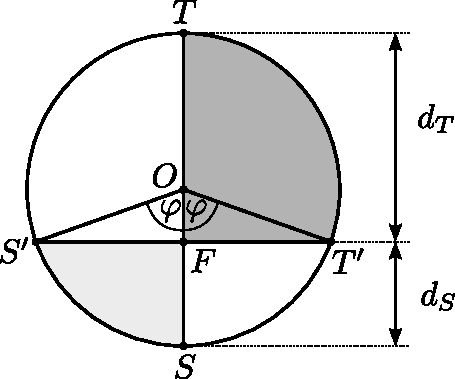
\includegraphics[width=0.4\linewidth]{2020-lahg-09-sol1.pdf}
\end{figure}

Edaspidi arvutame kõik pindalad ringiks venitatud ellipsi peal (vaata teist joonist), olgu ringi keskpunkt $O$.


Olgu Maa kaugused Päikesest suvisel ja talvisel pööripäeval vastavalt $d_S$ ja $d_T$. Vaatleme nüüd sfääre raadiustega $d_S$ ja $d_T$, mille keskpunktides on päike. Kuna sfääri pindala on proportsionaalne selle raadiuse ruuduga ning summaarne kiirgusenergia, mis jõuab kaugusele $d_T$ on sama, mis jõuab kaugusele $d_S$, siis järelikult on Päikese heledus pöördvõrdeline kauguse ruuduga. Seega saame, et
\[
\left(\frac{d_T}{d_S}\right)^2 = k^2 = \num{1.3},
\]
kus $k = \sqrt{\num{1.3}}$ on konstant valemite mugavamaks kirjapanekuks. Niisiis, $d_T = kd_S$.

\begin{figure}[H]
	\centering
	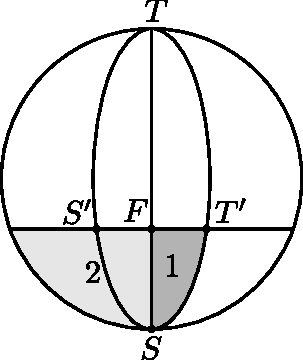
\includegraphics[width=0.6\linewidth]{2020-lahg-09-sol2.pdf}
\end{figure}

Ülejäänud ülesanne taandub geomeetria peale. $FSS'$ ja $FTT'$ pindalad on leitavad vastavate ringi sektorite ning kolmnurkade pindalade kaudu:
\begin{align*}
	T_S &= T_\oplus \frac{S_{FSS'}}{\pi R^2} = T_\oplus \frac{\frac{\varphi}{\ang{360}}\pi R^2 - \frac 12|OF||OS'|\sin\varphi}{\pi R^2}.\\
	&= T_\oplus \left(\frac{\varphi}{\ang{360}} - \frac{\cos\varphi\sin\varphi}{2\pi}\right),\\
\end{align*}
kus me asendasime $|OS'| = R$ ning $|OF| = |OS'|\cos\angle FOS' = R\cos\varphi$. Sarnaselt,
\[
T_T = T_\oplus \left(\frac{\ang{180} - \varphi}{\ang{360}} + \frac{\cos\varphi\sin\varphi}{2\pi}\right).
\]
$\varphi$ saame avaldada kui $\cos\varphi = |OF| / R = (R - d_S) / R$. Samas, $2R = d_T + d_S$, ehk $d_S = 2R/(1 + k)$ ning 
\[
\cos\varphi = 1 - \frac{2}{1 + k} = \frac{k - 1}{k + 1},
\]
ehk
\[
\varphi = \arccos\frac{k - 1}{k + 1} = \arccos\frac{\sqrt{\num{1.3}} - 1}{\sqrt{\num{1.3}} + 1} = \ang{86.24}.
\]
Niisiis, otsitav aegade vahe on 
\[
\Delta T = T_T - T_S = T_\oplus \left(\frac{1}{2} - \frac{\varphi}{\ang{180}} + \frac{\sin\varphi\cos\varphi}{\pi}\right) = \SI{15.2}{päeva}.
\]
\probend